\documentclass[11pt,a4paper]{article}

\usepackage{amsmath}
\usepackage{graphicx}
\usepackage{epstopdf}

\title{AMTH250 \\ Assignment 6}

\author{Mark Villar}

\begin{document}

\maketitle

\subsubsection*{Question 1} 
The basis functions are
\begin{align*}
	f_{1}(x)=e^{-2x}, \quad f_{2}(x)=e^{-x}, \quad f_{3}(x)=1, \quad f_{4}(x)=e^{x}, \quad f_{5}(x)=e^{2x}
\end{align*}
We determine the basis matrix and solve the following system in Octave.
\begin{align*}
	\begin{bmatrix}
		e^{4} &e^{2} &1 &e^{-2} &e^{-4} \\
		e^{2} &e &1 &e^{-1} &e^{-2} \\
		1 &1 &1 &1 &1\\
		e^{-2} &e^{-1} &1 &e &e^{2} \\
		e^{-4} &e^{-2} &1 &e^{2} &e^{4}
	\end{bmatrix} 
	\begin{bmatrix}
		a_{1} \\
		a_{2} \\
		a_{3} \\
		a_{4} \\
		a_{5}
	\end{bmatrix} =
	\begin{bmatrix}
		125.948 \\
		7.673 \\
		-4.000 \\
		-14.493 \\
		-103.429
	\end{bmatrix}
\end{align*}
The solution below gives us the coefficients of the basis functions.
\begin{center}
	\begin{tabular}{|c|c|}
	\hline
	Coefficient &Estimate \\
	\hline
	$a_1$ &3.0000 \\
	$a_2$ &-4.9998 \\
	$a_3$ &-1.0004 \\
	$a_4$ &1.0003 \\
	$a_5$ &-2.0000 \\
	\hline
	\end{tabular}
\end{center}
Thus the interpolation function is
\begin{align*}
	f(x)=3.00e^{-2x}-5.00e^{-x}-1.00+1.00e^{x}-2.00e^{2x}
\end{align*}

\pagebreak

\subsubsection*{Question 2}
\begin{enumerate}
	\item[(a)] \textit{Cubic spline interpolation}
	\begin{center}
		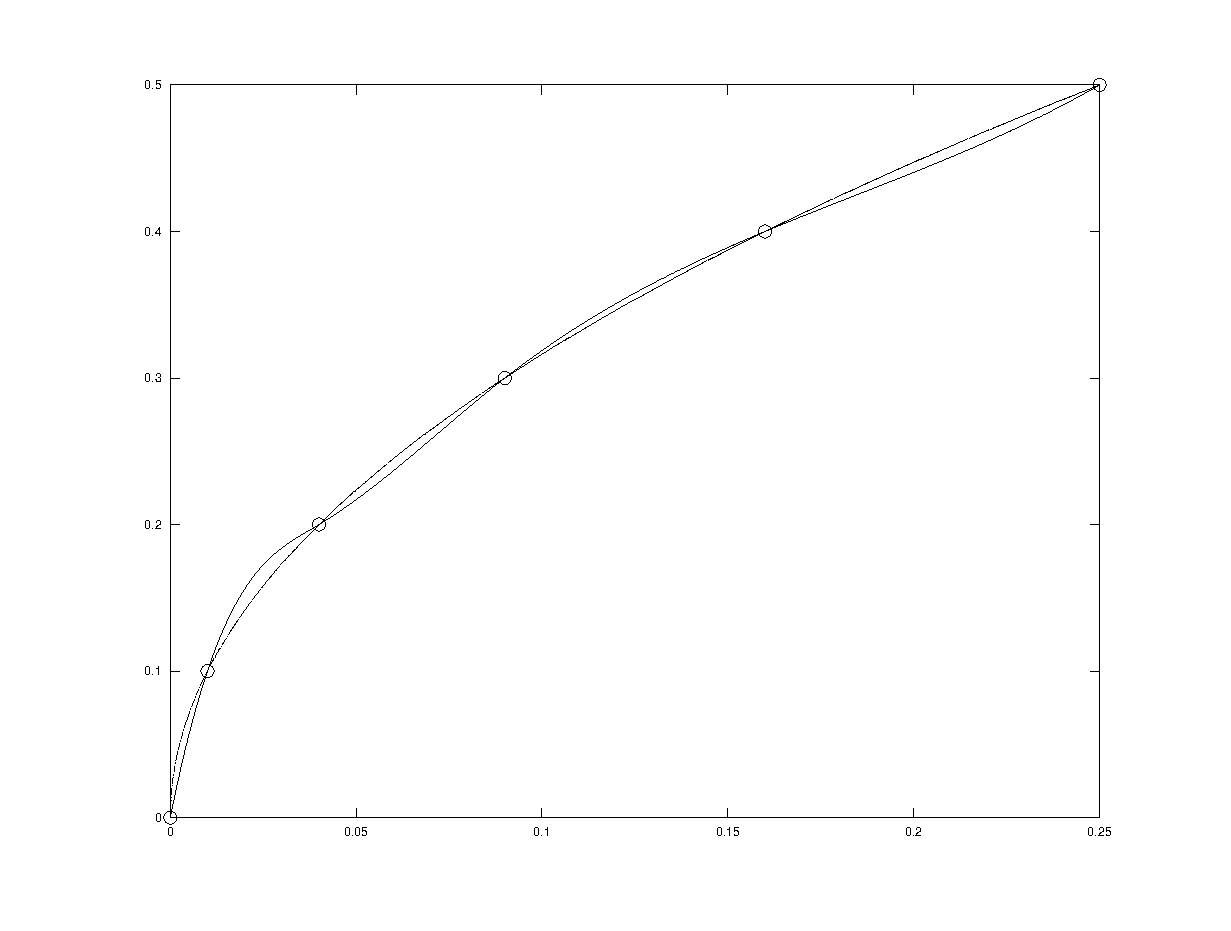
\includegraphics[width=0.5\textwidth]{cubicspline.eps}
	\end{center}
	\item[(b)] \textit{Pchip interpolation}
	\begin{center}
		\includegraphics[width=0.5\textwidth]{pchip.eps}
	\end{center}

	\item[(c)] \textit{Polynomial of degree 5}
	\begin{center}
		\includegraphics[width=0.5\textwidth]{poly5.eps}
	\end{center}
\end{enumerate}
The pchip interpolation is the most accurate over most of the domain. It is also the most accurate between 0 and 0.01.

\pagebreak

\subsubsection*{Question 3}
\begin{enumerate}
	\item[(a)] \textit{Cubic spline interpolation}
	\begin{center}
		\includegraphics[width=0.9\textwidth]{q3cs.eps}
	\end{center}
	
	\textit{Pchip interpolation}
	\begin{center}
		\includegraphics[width=0.9\textwidth]{q3pc.eps}
	\end{center}
	
	\item[(b)] Since the third derivatives in each case are piecewise constant, both interpolating functions are defined by a different cubic polynomial on each subinterval $[x_i,x_{i+1}]$. Since the first derivative of the cubic spline is smooth (and continuous) and its second derivative continuous, then at each interior knot, $x_2, \ldots , x_{n-1}$, the cubic polynomials on adjoining intervals have their values and the values of their first and second derivatives match. On the other hand,  the first derivative of the pchip displays kinks, which implies that the second derivative has jumps or discontinuities at the knots. This means that unlike the cubic spline, the condition that second derivatives match at the knots is dropped. The ``not-a-knot'' condition appears in the third derivative of the cubic spline, where the first two intervals and the last two intervals take on the same values.

\end{enumerate}

\subsubsection*{Question 4} The table below gives the least-squares solution to an overdetermined set of linear equations, where $x_i$ is the altitude with respect to some reference point.
	\begin{center}
		\begin{tabular}{|c|c|}
		\hline
		Coefficient &Estimate \\
		\hline
		$x_1$ &2.960 \\
		$x_2$ &0.554 \\
		$x_3$ &0.282 \\
		$x_4$ &0.764 \\
		\hline
		\end{tabular}
	\end{center}
Apart from $x_1$, the computed values are not at all accurate in comparison to the direct measurements. This is because we have more equations than unknowns. It follows that our matrix $\mathbf{B}$ has the property $n>k$, where $n=10$ and $k=4$. In such cases, a solution is not generally known.

\pagebreak

\subsubsection*{Question 5}

	\textit{Quadratic polynomial}
	$$f(x)=4.7027x^2-27.3516x+67.9317$$
	\begin{center}
		\includegraphics[width=0.5\textwidth]{qp.eps}
	\end{center}
	\textit{Power function}
	$$f(x)=18.679x^{0.91216}$$
	\begin{center}
		\includegraphics[width=0.5\textwidth]{pf.eps}
	\end{center}
	\textit{Exponential function}
	$$f(x)=19.212e^{0.24538x}$$
	\begin{center}
		\includegraphics[width=0.5\textwidth]{ef.eps}
	\end{center}
	The exponential function appears to give the best representation of the data, albeit marginally over the quadratic polynomial.
	
\subsubsection*{Question 6}
\begin{enumerate}
	\item[(a)] We only show polynomials fits for up to degree 4 since higher order approximations display only minimal improvements.
	
	\textit{Fits}
		\begin{center}
			\includegraphics[width=0.9\textwidth]{pfits.eps}
		\end{center}
	\textit{Residuals}
		\begin{center}
			\includegraphics[width=0.9\textwidth]{pres.eps}
		\end{center}
	\begin{enumerate}
		\item[(i)] By looking at the graphs above, all polynomial fits except the straight line captures the general trend of the data. From the graph of the residuals and their norms below, we may conclude that the best fit would be the quartic polynomial. However, we could also argue that the quadratic polynomial is best, by the rule of parsimony. 
		\begin{center}
			\begin{tabular}{|c|c|}
			\hline
			Degree &Norm \\
			\hline
			1 &86.356 \\
			2 &55.122 \\
			3 &54.979 \\
			4 &54.056 \\
			\hline
			\end{tabular}
		\end{center}
		\item[(ii)] We show the matrix of coefficients, where $c_0$ is the constant term, $c_1$ is the coefficient of the linear term and so on, for $n_{1m}$ where $m=1 \ldots 11$.

		\begin{verbatim}
			c0_c4 =
			347.34142    22.46708     0.00000     0.00000     0.00000
			344.40817    22.46708     2.93782     0.00000     0.00000
			344.40817    22.82652     2.93782     0.20000     0.00000
			344.85351    22.82652     1.45103     0.20000     0.57910
			344.85351    22.89047     1.45103     0.29964     0.57910
			345.13344    22.89047     0.51161     0.29964     2.54485
			345.13344    23.40518     0.51161     1.84624     2.54485
			345.25507    23.40518     1.97343     1.84624     5.22917
			345.25507    24.51666     1.97343     7.28895     5.22918
			345.22592    24.51666     1.43815     7.28896     3.68026
			345.22592    25.27155     1.43815    12.74995     3.68028
			
			c5_c10 =
			0.00000    0.00000    0.00000    0.00000    0.00000    0.00000
			0.00000    0.00000    0.00000    0.00000    0.00000    0.00000
			0.00000    0.00000    0.00000    0.00000    0.00000    0.00000
			0.00000    0.00000    0.00000    0.00000    0.00000    0.00000
			0.02994    0.00000    0.00000    0.00000    0.00000    0.00000
			0.02994    0.48128    0.00000    0.00000    0.00000    0.00000
			1.16592    0.48128    0.23478    0.00000    0.00000    0.00000
			1.16592    2.03471    0.23478    0.27784    0.00000    0.00000
			8.25292    2.03471    3.61501    0.27784    0.53293    0.00000
			8.25292    0.48326    3.61501    0.35115    0.53293    0.08867
			19.1930    0.48328   12.48587    0.35114    3.65931    0.08867
		\end{verbatim}
		\pagebreak
		We observe that the coefficients change as successively higher degree polynomials are fitted. Moreover, when an odd degree term is added it is mostly the odd degree lower order coefficients that change. Meanwhile, when an even degree term is added it is mostly the even degree lower order coefficients that change. This can be explained in terms of odd and even functions and how they behave when added together, as well as the fact that we centred our data.
		\end{enumerate}
		
	\item[(b)] The graphs below show the different model combinations we fitted.
	
		$n_1=1$
		\begin{center}
			\includegraphics[width=0.75\textwidth]{pt1.eps}
		\end{center}
		$n_1=2$
		\begin{center}
			\includegraphics[width=0.75\textwidth]{pt2.eps}
		\end{center}
		$n_1=4$
		\begin{center}
			\includegraphics[width=0.75\textwidth]{pt3.eps}
		\end{center}
		
	\begin{enumerate}
		\item[(i)] The graphs suggest that either a polynomial of degree 2 or 4 gives a much better fit than a straight line, which is consistent with our answer to part (a).  The trigonometric `degree' which combines best with the quadratic or quartic polynomial, however, is not so obvious. There seems to be very little difference in overall fit, regardless of the value of $n_2$.
		\item[(ii)] We look at the residual plots and their norms to determine which combination gives the best fit.
		\begin{center}
			\begin{tabular}{|c|c|c|}
			\hline
			$n_1$ &$n_2$ &Norm \\
			\hline
			2 &1 &22.826 \\
			2 &2 &18.266 \\
			2 &3 &18.205 \\
			2 &4 &18.167 \\
			4 &1 &20.589 \\
			4 &2 &15.356 \\
			4 &3 &15.291 \\
			4 &4 &15.244 \\
			\hline
			\end{tabular}
		\end{center}
		The table shows there is little improvement over trigonometric degree 2 for both the quadratic and quartic. So for parsimonious reasons we choose $n_2=2$, thereby avoiding the added complexity of estimating more coefficients and its associated errors. We then compare the residual plots for $n_1=2$ and $n_1=4$ below. While both are very similar, we choose the latter model due to its smaller norm and its slightly more stochastic pattern of its residuals.
			\begin{center}
			\includegraphics[width=0.85\textwidth]{ptres.eps}
		\end{center}
		
		\item[(iii)] We fix the polynomial degree $n_1$ at 4 and fit successively higher trig degree models for $n_{2m}$ where $m=1\ldots10$. The table of coefficients is shown below.
		
		\begin{verbatim}
			polyd0_d4 =
			5.2159e-001  1.9877e-001  1.5658e+000  2.2824e+001  3.4483e+002
			5.2191e-001  2.0253e-001  1.5651e+000  2.2829e+001  3.4483e+002
			5.2122e-001  2.0253e-001  1.5665e+000  2.2829e+001  3.4483e+002
			5.2122e-001  2.0291e-001  1.5665e+000  2.2830e+001  3.4483e+002
			5.2134e-001  2.0291e-001  1.5662e+000  2.2830e+001  3.4483e+002
			5.2128e-001  2.0316e-001  1.5664e+000  2.2830e+001  3.4483e+002
			5.2135e-001  2.0342e-001  1.5660e+000  2.2831e+001  3.4483e+002
			5.2167e-001  2.0266e-001  1.5650e+000  2.2829e+001  1.1071e+009
			5.2160e-001  2.0218e-001  1.5647e+000  2.2828e+001  1.0931e+009
			5.2289e-001  2.0330e-001  1.5621e+000  2.2830e+001  1.0940e+009
			
			sind1_d5 =
			1.7401e+000  0.0000e+000  0.0000e+000  0.0000e+000  0.0000e+000
			1.7430e+000  3.5868e-001  0.0000e+000  0.0000e+000  0.0000e+000
			1.7434e+000  3.5883e-001  3.2753e-002  0.0000e+000  0.0000e+000
			1.7436e+000  3.5883e-001  3.2276e-002  6.2568e-002  0.0000e+000
			1.7436e+000  3.5884e-001  3.2050e-002  6.2641e-002  1.8660e-002
			1.7437e+000  1.3527e+009  3.2031e-002  6.2625e-002  1.8415e-002
			1.8733e+009  1.3929e+009  8.1540e+008  6.3085e-002  7.2731e+010
			1.7343e+009  1.4855e+009  6.4259e+008  2.0594e+011  7.5059e+010
			2.3636e+009  1.2647e+009  2.7937e+011  1.9912e+011  8.2925e+010
			1.9165e+009  4.2467e+011  2.9627e+011  2.0279e+011  7.4368e+010
  
			sind6_d10 =
			0.0000e+000  0.0000e+000  0.0000e+000  0.0000e+000  0.0000e+000
			0.0000e+000  0.0000e+000  0.0000e+000  0.0000e+000  0.0000e+000
			0.0000e+000  0.0000e+000  0.0000e+000  0.0000e+000  0.0000e+000
			0.0000e+000  0.0000e+000  0.0000e+000  0.0000e+000  0.0000e+000
			0.0000e+000  0.0000e+000  0.0000e+000  0.0000e+000  0.0000e+000
			3.0642e-001  0.0000e+000  0.0000e+000  0.0000e+000  0.0000e+000
			3.1527e-001  7.2731e+010  0.0000e+000  0.0000e+000  0.0000e+000
			3.3582e-001  7.5059e+010  2.0703e+011  0.0000e+000  0.0000e+000
			2.8526e-001  7.8302e+010  2.0014e+011  2.8005e+011  0.0000e+000
			3.1934e+009  7.0057e+010  2.0386e+011  2.9718e+011  4.2292e+011
			
			cosd1_d5 =
			2.1817e+000  0.0000e+000  0.0000e+000  0.0000e+000  0.0000e+000
			2.1791e+000  6.7718e-001  0.0000e+000  0.0000e+000  0.0000e+000
			2.1792e+000  6.7772e-001  7.1500e-002  0.0000e+000  0.0000e+000
			2.1792e+000  6.7772e-001  7.1389e-002  2.4747e-002  0.0000e+000
			2.1793e+000  6.7766e-001  7.1464e-002  2.4614e-002  1.6239e-002
			2.1792e+000  7.8096e+008  7.1445e-002  2.4385e-002  1.6328e-002
			1.4000e+008  8.0420e+008  1.6923e+009  2.4105e-002  1.0672e+011
			2.5933e+008  8.5766e+008  1.6317e+009  2.0224e+011  9.4348e+010
			5.2887e+009  7.3020e+008  2.0702e+011  1.9239e+011  9.6759e+010
			5.0487e+009  4.6390e+009  1.7240e+011  1.9864e+011  1.1007e+011
  
			cosd6_d10 =
			0.0000e+000  0.0000e+000  0.0000e+000  0.0000e+000  0.0000e+000
			0.0000e+000  0.0000e+000  0.0000e+000  0.0000e+000  0.0000e+000
			0.0000e+000  0.0000e+000  0.0000e+000  0.0000e+000  0.0000e+000
			0.0000e+000  0.0000e+000  0.0000e+000  0.0000e+000  0.0000e+000
			0.0000e+000  0.0000e+000  0.0000e+000  0.0000e+000  0.0000e+000
			1.0738e+011  0.0000e+000  0.0000e+000  0.0000e+000  0.0000e+000
			1.1058e+011  1.0672e+011  0.0000e+000  0.0000e+000  0.0000e+000
			1.1793e+011  9.4348e+010  2.0635e+011  0.0000e+000  0.0000e+000
			1.0040e+011  9.8794e+010  1.9634e+011  2.0532e+011  0.0000e+000
			9.0805e+010  1.1257e+011  2.0268e+011  1.7070e+011  9.3356e+009
		\end{verbatim}
		
	\pagebreak
	The polynomial coefficients remain almost the same with the exception of the quadratic coefficient for trig degrees $n_2 \ge 8$. The size of the coefficient increases dramatically from 344.83 to $\approx 1.1 \times 10^9$. Apart from this, the result is not surprising given the polynomial degree is fixed. On the other hand, trignometric coefficients tend to stay the same only for smaller $n_2$ degrees, with the size of some coefficients increasing dramatically as more trig terms are added. We also observe a similar kind of effect as in part (a)[ii] in terms of odd and even degree trig terms and how they interact when added together.
	\end{enumerate} 
	\item[(c)] Because of the oscillations in the data we must add periodic terms by way of trigonometric functions. Since these functions are nonlinear in the parameters, our design matrix would have been ill-conditioned had we not strandardised or rescaled the time data to account for such periodicity.
	\item[(d)] The residuals plot of our final model appears to show a significant drop in level around the year 1991, which could be a result of a particular event or `shock' that has impacted on the model. It may be worthwhile dividing the data into two distinct time periods and use separable least squares or step-function modelling.
\end{enumerate}

\pagebreak

\textbf{Appendix}

\begin{enumerate}

	\item
	\begin{verbatim}
		%determines the coefficients of an interpolating function
		x=[-2 -1 0 1 2]';
		aa=[exp(-2*x) exp(-x) ones(5,1) exp(x) exp(2*x)]
		b=[125.948 7.673 -4.000 -14.493 -103.429]'
		a=aa\b	
	\end{verbatim}

	\item
	\begin{enumerate}
		\item
		\begin{verbatim}
			%interpolates the square root function using a cubic spline
			xx=[0 .01 .04 .09 .16 .25];
			yy=[0 .1 .2 .3 .4 .5];
			x=linspace(0,.25,917);
			y=sqrt(x);
			pp=interp1(xx,yy,'spline','pp');
			plot(x,ppval(pp,x),x,y)
			hold on
			plot(xx,yy,'ro')
			print('cubicspline.eps','-deps')
		\end{verbatim}
		
		\item
		\begin{verbatim}
			%interpolates the square root function using a pchip cubic 
			pp=interp1(xx,yy,'pchip','pp');
			plot(x,ppval(pp,x),x,y)
			axis([0,.25,0,.5])
			hold on
			plot(xx,yy,'ro')
			print('pchip.eps','-deps')
		\end{verbatim}
		
		\item
		\begin{verbatim}
			%interpolates the square root function using a polynomial
			%of degree 5 
			p=polyfit(xx,yy,5)
			px=polyval(p,x);
			plot(x,px,x,y)
			hold on
			plot(xx,yy,'ro')
			print('poly5.eps','-deps')
		\end{verbatim}
		
	\end{enumerate}
	
	\item	
		\begin{verbatim}
			%computes and plots the cubic spline interpolants
			%and their first, second and third derivatives
			xx=1:1:7;
			yy=[1.9 2.7 4.8 5.3 7.1 9.4 11.3];
			pp=interp1(xx,yy,'spline','pp');
			x=linspace(1,7,917);
			subplot(2,2,1)
			plot(x,ppval(pp,x))
			hold on
			plot(xx,yy,'ro')
			title('Cubic spline')
			pp1=ppderiv(pp);
			subplot(2,2,2)
			plot(x,ppval(pp1,x))
			title('First derivative')
			pp2=ppderiv(pp1);
			subplot(2,2,3)
			plot(x,ppval(pp2,x))
			xlabel('Second derivative')
			pp3=ppderiv(pp2);
			subplot(2,2,4)
			plot(x,ppval(pp3,x))
			xlabel('Third derivative')
			print('q3cs.eps','-deps')
			
			%computes and plots the pchip interpolants and
			%their first, second and third derivatives
			pp=interp1(xx,yy,'pchip','pp');
			subplot(2,2,1)
			plot(x,ppval(pp,x))
			hold on
			plot(xx,yy,'ro')
			title('Pchip')
			pp1=ppderiv(pp);
			subplot(2,2,2)
			plot(x,ppval(pp1,x))
			title('First derivative')
			pp2=ppderiv(pp1);
			subplot(2,2,3)
			plot(x,ppval(pp2,x))
			xlabel('Second derivative')
			pp3=ppderiv(pp2);
			subplot(2,2,4)
			plot(x,ppval(pp3,x))
			xlabel('Third derivative')
			print('q3pc.eps','-deps')
		\end{verbatim}
	
	\item
		\begin{verbatim}
			%solves an overdetermined set of linear equations
			b=zeros(10,4);
			y=zeros(10,1);

			b(1,1)=1;
			y(1)=2.95;
			
			b(2,2)=1;
			y(2)=1.74;

			b(3,3)=1;
			y(3)=-1.45;

			b(4,4)=1;
			y(4)=1.32;

			b(5,1)=1;
			b(5,2)=-1;
			y(5)=1.23;

			b(6,1)=1;
			b(6,3)=-1;
			y(6)=4.45;

			b(7,1)=1;
			b(7,4)=-1;
			y(7)=1.61;

			b(8,2)=1;
			b(8,3)=-1;
			y(8)=3.21;

			b(9,2)=1;
			b(9,4)=-1;
			y(9)=0.45;

			b(10,3)=1;
			b(10,4)=-1;
			y(8)=-2.75;
			
			a=b\y
		\end{verbatim}

	\item
		\begin{verbatim}
			%fits a quadratic polynomial to a given set of data
			x=(1:10)';
			y=[27.7 39.3 38.4 57.6 46.3 54.8 108.5 137.6 194.1 281.2]';
			p=polyfit(x,y,2)
			plot(x,y,'ro')
			hold on
			xx=linspace(1,10,201)';
			plot(xx,polyval(p,xx))
			print('qp.eps','-deps')
		\end{verbatim}
		
		\begin{verbatim}
			%fits a power function to a given set of data
			s=polyfit(log(x),log(y),1)
			plot(x,y,'ro')
			hold on
			yy=e^s(2)*xx.^s(1);
			plot(xx,yy)
			print('pf.eps','-deps')
		\end{verbatim}
		
		\begin{verbatim}
			%fits an exponential function to a given set of data
			r=polyfit(x,log(y),1)
			plot(x,y,'ro')
			hold on
			xx=linspace(1,10,201)';
			yy=e^r(2)*exp(r(1)*xx);
			plot(xx,yy)
			print('ef.eps','-deps')
		\end{verbatim}
	
	\item
	\begin{enumerate}
		\item
		\begin{verbatim}
			%reads in data
			co2=load('co2_mm_mlo.txt');
			t=co2(:,3);
			conc=co2(:,5);

			%rescale time and computes constant k
			tt=(t-mean(t))/std(t);
			k=2*pi*std(t)

			%polynomial fits for up to degree 4
			[a10 c10]=polytrig(tt,conc,k,1,0);
			subplot(2,2,1)
			plot(t,conc)
			hold on
			plot(t,c10,'r')
			title('Straight line')
			hold off

			[a20 c20]=polytrig(tt,conc,k,2,0);
			subplot(2,2,2)
			plot(t,conc)
			hold on
			plot(t,c20,'r')
			title('Quadratic')
			hold off


			[a30 c30]=polytrig(tt,conc,k,3,0);
			subplot(2,2,3)
			plot(t,conc)
			hold on
			plot(t,c30,'r')
			xlabel('Cubic')
			hold off

			[a40 c40]=polytrig(tt,conc,k,4,0);
			subplot(2,2,4)
			plot(t,conc)
			hold on
			plot(t,c40,'r')
			xlabel('Quartic')
			hold off

			print('pfits.eps','-deps')

			subplot(2,2,1)
			r10=conc-c10;
			plot(t,r10)
			title('Straight line')
			subplot(2,2,2)
			r20=conc-c20;
			plot(t,r20)
			title('Quadratic')
			subplot(2,2,3)
			r30=conc-c30;
			plot(t,r30)
			xlabel('Cubic')
			subplot(2,2,4)
			r40=conc-c40;
			plot(t,r40)
			xlabel('Quartic')

			print('pres.eps','-deps')
		\end{verbatim}

		\begin{enumerate}
			\item[(i)]
			\begin{verbatim}
				%norms of the residuals
				norm(r10)
				norm(r20)
				norm(r30)
				norm(r40)
			\end{verbatim}
			
			\pagebreak
			
			\item[(ii)]
			\begin{verbatim}
				%fits higher order polynomials to the data
				[a50 c50]=polytrig(tt,conc,k,5,0);
				[a60 c60]=polytrig(tt,conc,k,6,0);
				[a70 c70]=polytrig(tt,conc,k,7,0);
				[a80 c80]=polytrig(tt,conc,k,8,0);
				[a90 c90]=polytrig(tt,conc,k,9,0);
				[a100 c100]=polytrig(tt,conc,k,10,0);
				[a110 c110]=polytrig(tt,conc,k,11,0);
				
				%creates matrix of coefficients
				c0=abs([a10(2) a20(3) a30(4) a40(5) a50(6) a60(7) a70(8) 
				a80(9) a90(10) a100(11) a110(12)])';
				c1=abs([a10(1) a20(2) a30(3) a40(4) a50(5) a60(6) a70(7) 
				a80(8) a90(9) a100(10) a110(11)])';
				c2=abs([0 a20(1) a30(2) a40(3) a50(4) a60(5) a70(6) a80(7) 
				a90(8) a100(9) a110(10)])';
				c3=abs([0 0 a30(1) a40(2) a50(3) a60(4) a70(5) a80(6) a90(7) 
				a100(8) a110(9)])';
				c4=abs([0 0 0 a40(1) a50(2) a60(3) a70(4) a80(5) a90(6) 
				a100(7) a110(8)])';
				c5=abs([0 0 0 0 a50(1) a60(2) a70(3) a80(4) a90(5) a100(6) 
				a110(7)])';
				c6=abs([0 0 0 0 0 a60(1) a70(2) a80(3) a90(4) a100(5) 
				a110(6)])';
				c7=abs([0 0 0 0 0 0 a70(1) a80(2) a90(3) a100(4) a110(5)])';
				c8=abs([0 0 0 0 0 0 0 a80(1) a90(2) a100(3) a110(4)])';
				c9=abs([0 0 0 0 0 0 0 0 a90(1) a100(2) a110(3)])';
				c10=abs([0 0 0 0 0 0 0 0 0 a100(1) a110(2)])';
				c11=abs([0 0 0 0 0 0 0 0 0 0 a110(1)])';
				coef=[c11 c10 c9 c8 c7 c6 c5 c4 c3 c2 c1 c0]
				c0_c4=[coef(:,12) coef(:,11) coef(:,10) coef(:,9) coef(:,8)]
				c5_c10=[coef(:,7) coef(:,6) coef(:,5) coef(:,4) coef(:,3) 
				coef(:,2)]
			\end{verbatim}
			
		\end{enumerate}
		
		\item
		\begin{enumerate}
		\begin{verbatim}
			%polytrig fits to the data
			[a11 c11]=polytrig(tt,conc,k,1,1);
			[a12 c12]=polytrig(tt,conc,k,1,2);
			[a13 c13]=polytrig(tt,conc,k,1,3);
			[a14 c14]=polytrig(tt,conc,k,1,4);
			
			[a21 c21]=polytrig(tt,conc,k,2,1);
			[a22 c22]=polytrig(tt,conc,k,2,2);
			[a23 c23]=polytrig(tt,conc,k,2,3);
			[a24 c24]=polytrig(tt,conc,k,2,4);
			
			[a41 c41]=polytrig(tt,conc,k,4,1);
			[a42 c42]=polytrig(tt,conc,k,4,2);
			[a43 c43]=polytrig(tt,conc,k,4,3);
			[a44 c44]=polytrig(tt,conc,k,4,4);
			
		\end{verbatim}

			\item[(i)]
			\begin{verbatim}
				%graphs of polytrig fits
				subplot(2,2,1)
				plot(t,conc)
				hold on
				plot(t,c11,'r')
				title('n2=1')
				hold off

				subplot(2,2,2)
				plot(t,conc)
				hold on
				plot(t,c12,'r')
				title('n2=2')
				hold off

				subplot(2,2,3)
				plot(t,conc)
				hold on
				plot(t,c13,'r')
				xlabel('n2=3')
				hold off

				subplot(2,2,4)
				plot(t,conc)
				hold on
				plot(t,c14,'r')
				xlabel('n2=4')
				hold off
				print('pt1.eps','-deps')

				subplot(2,2,1)
				plot(t,conc)
				hold on
				plot(t,c21,'r')
				title('n2=1')
				hold off

				subplot(2,2,2)
				plot(t,conc)
				hold on
				plot(t,c22,'r')
				title('n2=2')
				hold off

				subplot(2,2,3)
				plot(t,conc)
				hold on
				plot(t,c23,'r')
				xlabel('n2=3')
				hold off

				subplot(2,2,4)
				plot(t,conc)
				hold on
				plot(t,c24,'r')
				xlabel('n2=4')
				hold off
				print('pt2.eps','-deps')

				subplot(2,2,1)
				plot(t,conc)
				hold on
				plot(t,c41,'r')
				title('n2=1')
				hold off

				subplot(2,2,2)
				plot(t,conc)
				hold on
				plot(t,c42,'r')
				title('n2=2')
				hold off

				subplot(2,2,3)
				plot(t,conc)
				hold on
				plot(t,c43,'r')
				xlabel('n2=3')
				hold off


				subplot(2,2,4)
				plot(t,conc)
				hold on
				plot(t,c44,'r')
				xlabel('n2=4')
				hold off
				print('pt3.eps','-deps')
			\end{verbatim}
			
			\item[(ii)]
			\begin{verbatim}
				%norms of the polytrig residuals
				r21=conc-c21;
				norm(r21)
				r22=conc-c22;
				norm(r22)
				r23=conc-c23;
				norm(r23)
				r24=conc-c24;
				norm(r24)

				r41=conc-c41;
				norm(r41)
				r42=conc-c42;
				norm(r42)
				r43=conc-c43;
				norm(r43)
				r44=conc-c44;
				norm(r44)
				
				subplot(2,1,1)
				plot(t,r22)
				title('n1=2, n2=2')

				subplot(2,1,2)
				plot(t,r42)
				xlabel('n1=4, n2=2')
				print('ptres.eps','-deps')
				
			\end{verbatim}
			
			\item[(iii)]
			\begin{verbatim}
				%higher order polytrig fits with polynomial degree fixed
				[a45 c45]=polytrig(tt,conc,k,4,5);
				[a46 c46]=polytrig(tt,conc,k,4,6);
				[a47 c47]=polytrig(tt,conc,k,4,7);
				[a48 c48]=polytrig(tt,conc,k,4,8);
				[a49 c49]=polytrig(tt,conc,k,4,9);
				[a410 c410]=polytrig(tt,conc,k,4,10);
			
				d4=abs([a41(1) a42(1) a43(1) a44(1) a45(1) a46(1) a47(1) 
				a48(1) a49(1) a410(1)])';
				d3=abs([a41(2) a42(2) a43(2) a44(2) a45(2) a46(2) a47(2) 
				a48(2) a49(2) a410(2)])';
				d2=abs([a41(3) a42(3) a43(3) a44(3) a45(3) a46(3) a47(3) 
				a48(3) a49(3) a410(3)])';
				d1=abs([a41(4) a42(4) a43(4) a44(4) a45(4) a46(4) a47(4) 
				a48(4) a49(4) a410(4)])';
				d0=abs([a41(5) a42(5) a43(5) a44(5) a45(5) a46(5) a47(5) 
				a48(5) a49(5) a410(5)])';

				ds1=abs([a41(6) a42(6) a43(6) a44(6) a45(6) a46(6) a47(6) 
				a48(6) a49(6) a410(6)])';
				dc1=abs([a41(7) a42(7) a43(7) a44(7) a45(7) a46(7) a47(7) 
				a48(7) a49(7) a410(7)])';
				ds2=abs([0 a42(8) a43(8) a44(8) a45(8) a46(8) a47(8) a48(8) 
				a49(8) a410(8)])';
				dc2=abs([0 a42(9) a43(9) a44(9) a45(9) a46(9) a47(9) a48(9) 
				a49(9) a410(9)])';
				ds3=abs([0 0 a43(10) a44(10) a45(10) a46(10) a47(10) a48(10) 
				a49(10) a410(10)])';
				dc3=abs([0 0 a43(11) a44(11) a45(11) a46(11) a47(11) a48(11) 
				a49(11) a410(11)])';
				ds4=abs([0 0 0 a44(12) a45(12) a46(12) a47(12) a48(12) a49(12) 
				a410(12)])';
				dc4=abs([0 0 0 a44(13) a45(13) a46(13) a47(13) a48(13) a49(13) 
				a410(13)])';
				ds5=abs([0 0 0 0 a45(14) a46(14) a47(14) a48(14) a49(14) 
				a410(14)])';
				dc5=abs([0 0 0 0 a45(15) a46(15) a47(15) a48(15) a49(15) 
				a410(15)])';
				ds6=abs([0 0 0 0 0 a46(16) a47(16) a48(16) a49(16) a410(16)])';
				dc6=abs([0 0 0 0 0 a46(17) a47(17) a48(17) a49(17) a410(17)])';
				ds7=abs([0 0 0 0 0 0 a47(18) a48(18) a49(18) a410(18)])';
				dc7=abs([0 0 0 0 0 0 a47(19) a48(19) a49(19) a410(19)])';
				ds8=abs([0 0 0 0 0 0 0 a48(20) a49(20) a410(20)])';
				dc8=abs([0 0 0 0 0 0 0 a48(21) a49(21) a410(21)])';
				ds9=abs([0 0 0 0 0 0 0 0 a49(22) a410(22)])';
				dc9=abs([0 0 0 0 0 0 0 0 a49(23) a410(23)])';
				ds10=abs([0 0 0 0 0 0 0 0 0 a410(24)])';
				dc10=abs([0 0 0 0 0 0 0 0 0 a410(25)])';



				polyd0_d4=[d4 d3 d2 d1 d0]
				sind1_d5=[ds1 ds2 ds3 ds4 ds5]
				sind6_d10=[ds6 ds7 ds8 ds9 ds10]
				cosd1_d5=[dc1 dc2 dc3 dc4 dc5]
				cosd6_d10=[dc6 dc7 dc8 dc9 dc10]
			\end{verbatim}
			
		\end{enumerate}
	\end{enumerate}
	
\end{enumerate}

\end{document}